\documentclass{ximera}  

\title{The Cross Product}  

\begin{document}  
\begin{abstract}  
%abstract
\end{abstract}  
\maketitle 

In this section, we review the vector cross product, including the geometric perspective of the cross product, the area of a parallelogram, and the volume of parallelepiped.

\section{The Cross Product}

The cross product is fundamentally different from the dot product in a couple of ways. The cross product is defined only on vectors in $\mathbb{R}^3$, while the dot product is defined in $\mathbb{R}^n$ for any positive integer $n$. Furthermore, the cross product takes two vectors and produces another vector, while the dot product takes two vectors and produces a scalar.

We now give the algebraic definition of the cross product.

\begin{definition}
Let $\vec{a}=(a_1,a_2,a_3)$ and $\vec{b}=(b_1,b_2,b_3)$ be vectors in $\mathbb{R}^3$. The \emph{cross product} of $\vec{a}$ and $\vec{b}$, denoted $\vec{a}\times\vec{b}$, is defined to be
\[
\vec{a}\times\vec{b}=\left(\begin{array}{c}a_2b_3-a_3b_2\\a_3b_1-a_1b_3\\a_1b_2-a_2b_1\end{array}\right).
\]
Equivalently, we can compute the cross product as
\[
\vec{a}\times\vec{b}=\textrm{det}\left(\begin{array}{ccc}\mathbf{i}&\mathbf{j}&\mathbf{k}\\a_1&a_2&a_3\\b_1&b_2&b_3\end{array}\right),
\]
where
\begin{align*}
\mathbf{i}&=(1,0,0),\\
\mathbf{j}&=(0,1,0),\\
\mathbf{k}&=(0,0,1).
\end{align*}
\end{definition}

\begin{example}
\begin{align*}
(3,2,-1)\times(9,0,2) &= \textrm{det}\left(\begin{array}{ccc}\textbf{i}&\textbf{j}&\textbf{k}\\3&2&-1\\9&0&2\end{array}\right)\\
&= (2\cdot 2)\mathbf{i} - (0\cdot -1)\mathbf{i} + (-1\cdot 9)\mathbf{j} - (2\cdot 3)\mathbf{j}+(3\cdot 0)\mathbf{k} - (9\cdot -1)\mathbf{k}\\
&= 4\mathbf{i}-15\mathbf{j}+9\mathbf{k}\\
&= (4,-15, 9)
\end{align*}
\end{example}

The cross product has some nice algebraic properties, which can be very useful.

\begin{proposition}
Let $\vec{a}$, $\vec{b}$, and $\vec{c}$ be vectors in $\mathbb{R}^3$, and let $k\in\mathbb{R}$ be a scalar. The cross product has the following properties:
\begin{enumerate}
\item $\vec{a}\times \vec{b} = -\vec{b}\times \vec{a}$ (the cross product is \emph{anticommutative});
\item $\vec{a}\times(\vec{b}+\vec{c}) = \vec{a}\times\vec{b}+\vec{a}\times\vec{c}$;
\item $(\vec{a}+\vec{b})\times\vec{c} = \vec{a}\times\vec{c}+\vec{b}\times\vec{c}$ (with the previous property, the cross product is \emph{distributive} over vector addition);
\item $k(\vec{a}\times\vec{b})=(k\vec{a})\times\vec{b} = \vec{a}\times(k\vec{b})$.
\end{enumerate}
\end{proposition}

In particular, it's important to remember that the cross product is \emph{not} commutative, so the order of the vectors matters!

\section{Geometry of the Cross Product}

It's often easiest to compute cross products algebraically, but it's easier to understand their significance from a geometric perspective. We now discuss some of the geometric properties of the cross product.

\begin{proposition}
Let $\vec{a}$ and $\vec{b}$ be vectors in $\mathbb{R}^3$, and consider their cross product $\vec{a}\times\vec{b}$.
\begin{itemize}
\item The \emph{magnitude} of the vector $\vec{a}\times\vec{b}$ can be computed as 
\[
\|\vec{a}\times\vec{b}\| = \|\vec{a}\|\,\|\vec{b}\|\sin(\theta),
\]
where $\theta$ is the angle between the vectors $\vec{a}$ and $\vec{b}$. Furthermore, this magnitude is equal to the area of the parallelogram determined by $\vec{a}$ and $\vec{b}$.

\begin{image}
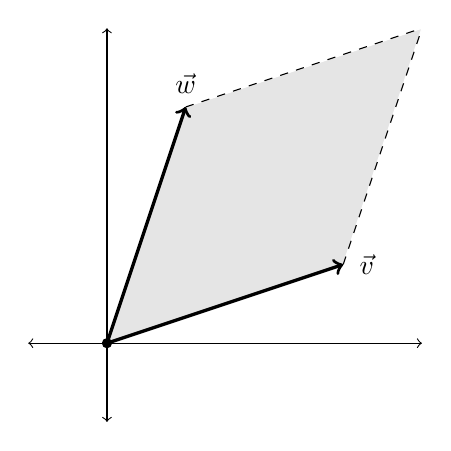
\begin{tikzpicture}
\draw[<->] (-1,0) -- (4,0);
\draw[<->] (0,-1) -- (0,4);

\draw[white, fill=gray!20] (0,0) -- (1,3) -- (4,4) -- (3,1) --  cycle;

\node[draw, circle, thick, fill=black, minimum size=1mm, inner sep=0] at (0,0) {};
\draw[->, very thick] (0,0) -- (1,3);
\draw[->,very thick] (0,0) -- (3,1);
\draw[dashed] (1, 3) -- (4, 4);
\draw[dashed] (3, 1) -- (4,4);

\node at (3.3,1) {$\vec{v}$};
\node at (1,3.3) {$\vec{w}$};

\end{tikzpicture}
\end{image}

\item The vector $\vec{a}\times\vec{b}$ is always perpendicular to both $\vec{a}$ and $\vec{b}$, and follows the \emph{right-hand rule}. That is, if you take your right hand and orient it so you can curl your fingers from the vector $\vec{a}$ to the $\vec{b}$, your thumb will be pointing in the same direction as the cross product $\vec{a}\times\vec{b}$.

\begin{image}
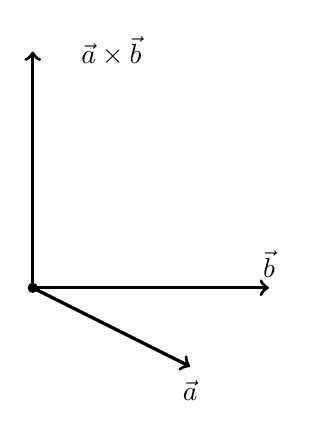
\begin{tikzpicture}

\node[draw, circle, thick, fill=black, minimum size=1mm, inner sep=0] at (0,0) {};
\draw[->, very thick] (0,0) -- (3,0);
\draw[->,very thick] (0,0) -- (2,-1);
\draw[->,very thick] (0,0) -- (0,3);

\node at (3,0.3) {$\vec{b}$};
\node at (2,-1.3) {$\vec{a}$};
\node at (1,3) {$\vec{a}\times\vec{b}$};

\end{tikzpicture}
\end{image}

Image this image in $\mathbb{R}^3$, so that $\vec{a}\times\vec{b}$ is perpendicular to both $\vec{a}$ and $\vec{b}$.

\end{itemize}
\end{proposition}

\section{Volume of a Parallelepiped}

We can use the cross product and dot product together to compute the volume of a parallelepiped.

\begin{image}
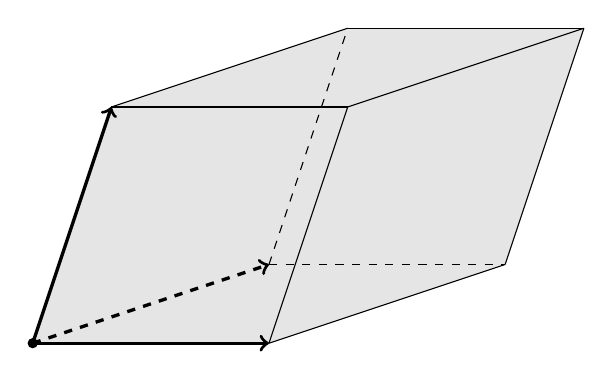
\begin{tikzpicture}

\draw[white, fill=gray!20] (0,0) -- (3,0) -- (6,1) -- (7,4) -- (4,4) -- (1,3) --  cycle;

\node[draw, circle, thick, fill=black, minimum size=1mm, inner sep=0] at (0,0) {};
\draw[->, very thick] (0,0) -- (3,0);
\draw[->, dashed, very thick] (0,0) -- (3,1);
\draw[->,very thick] (0,0) -- (1,3);
\draw[] (3, 0) -- (4, 3);
\draw[] (1, 3) -- (4,3);
\draw[] (1, 3) -- (4,4);
\draw[] (3, 0) -- (6,1);
\draw[] (4, 3) -- (7,4);
\draw[] (6, 1) -- (7,4);
\draw[] (4, 4) -- (7,4);
\draw[dashed] (3,1) -- (6,1);
\draw[dashed] (3,1) -- (4,4);

\end{tikzpicture}
\end{image}

The volume of the parellelepiped can be computed as the area of the base times the height. We've seen that the area of the base can be computed as the magnitude of a cross product, $\|\vec{a}\times\vec{b}\|$. The height of the parallelepiped can be computed as $\|\vec{c}\|\,|\cos(\theta)|$, where $\theta$ is the angle between the vector $\vec{c}$ and a line perpendicular to the base. We then have that the volume is $\|\vec{a}\times\vec{b}\|\,\|\vec{c}\|\,|\cos(\theta)|$, which we can recognize as the absolute value of the dot product of the vectors $\vec{a}\times\vec{b}$ and $\vec{c}$. Thus we have the following proposition.

\begin{proposition}
The volume of the parallelepiped determined by the vectors $\vec{a}$, $\vec{b}$, and $\vec{c}$ can be computed as $|(\vec{a}\times\vec{b})\cdot\vec{c}|$.
\end{proposition}

\section{Summary}

We've reviewed the cross product, including its properties and geometric perspective, including its use in finding the area of parallelograms and volume of parallelepipeds.

\end{document}